\documentclass{beamer}
\beamertemplatenavigationsymbolsempty
\usecolortheme{beaver}
\setbeamertemplate{blocks}[rounded=true, shadow=true]
\setbeamertemplate{footline}[page number]
%
\usepackage[utf8]{inputenc}
\usepackage[english,russian]{babel}
\usepackage{amssymb,amsfonts,amsmath,mathtext}
\usepackage{subfig}
\usepackage[all]{xy} % xy package for diagrams
\usepackage{array}
\usepackage{multicol}% many columns in slide
\usepackage{hyperref}% urls
\usepackage{hhline}%tables
\usepackage{svg}
% Your figures are here:
\graphicspath{ {../figures/} }

%----------------------------------------------------------------------------------------------------------
\title[\hbox to 56mm{Тема}]{Выбор интерпретируемых рекуррентных моделей глубокого обучения}
\author[Н.\,П. Ивкин]{Гапонов Максим}
\institute{Московский физико-технический институт}
\date{\footnotesize
% \par\smallskip\emph{Курс:} Автоматизация научных исследований\par (практика, В.\,В.~Стрижов)/Группа 874
\par\smallskip\emph{Эксперт:} Бахтеев Олег
\par\smallskip\emph{Консультант:} Яковлев Константин
\par\bigskip\small 2022}
%----------------------------------------------------------------------------------------------------------
\begin{document}
%----------------------------------------------------------------------------------------------------------
\begin{frame}
\thispagestyle{empty}
\maketitle
\end{frame}
%-----------------------------------------------------------------------------------------------------
\begin{frame}{Цель исследования}
Решается задача выбора интерпретируемых рекуррентных моделей.
\bigskip

Требуется найти метод получения интерпретаций предсказаний произвольной рекуррентной модели глубокого обучения с кусочно-линейными функциями активации.
\bigskip

Предлагается обобщить ранее известный метод OpenBox, который предназначен для обыкновенных нейронных сетей с кусочно-линейными функциями активации.
\end{frame}
%-----------------------------------------------------------------------------------------------------
\begin{frame}{Выбор интерпретируемых рекуррентных моделей}

Получение интерпретации предсказаний модели глубокого обучения необходимо для того, чтобы эксперты в различных областях могли "доверять" модели и принимать решения на основе её предсказаний.

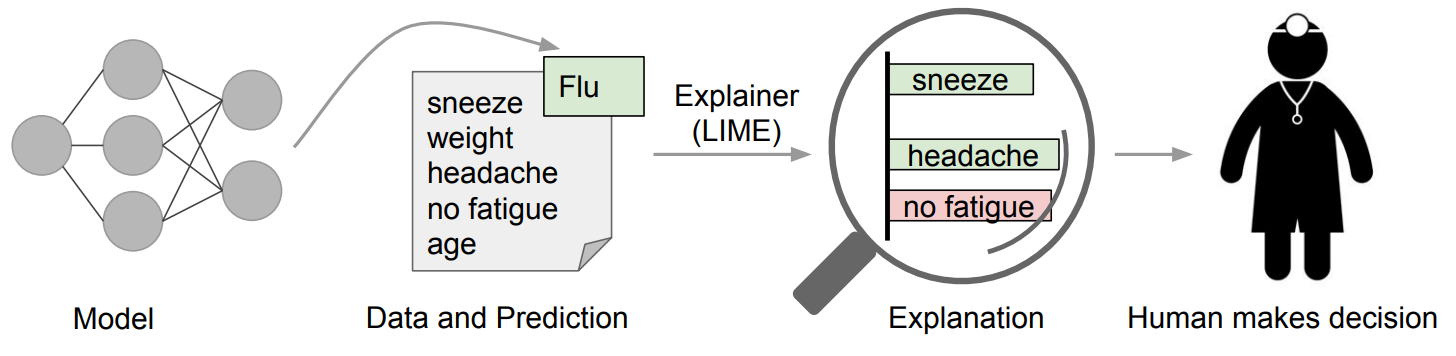
\includegraphics[width=\textwidth]{../figures/lime_int_exp.png}

Интерпретация должна быть {\color{red}\textbf{точной}}, то есть поведение интерпретируемой модели похоже на исходную модель, и {\color{red}\textbf{согласованной}}, то есть интерпретации близких объектов должны быть похожи.

% Требуется выбрать интерпретируемую \textbf{рекуррентную} модель глубокого обучения.
% 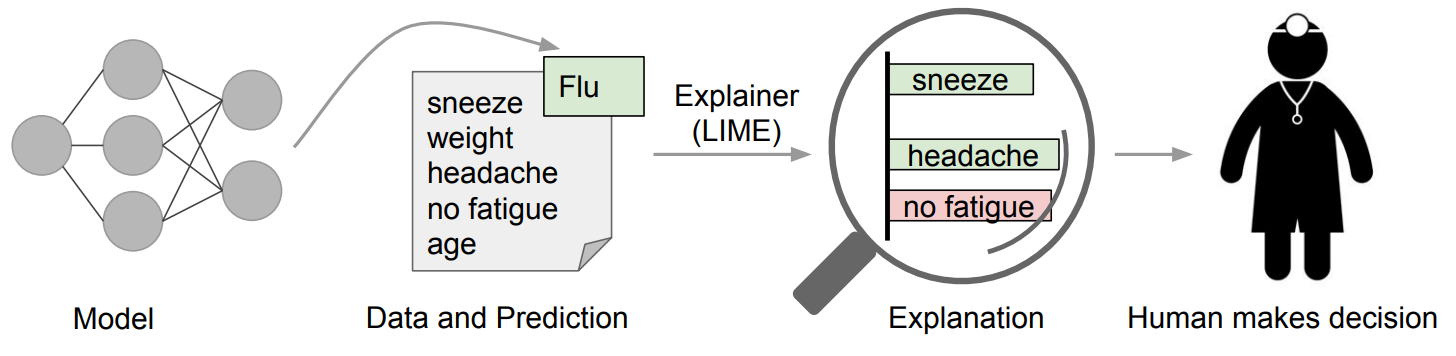
\includegraphics[width=10cm]{../figures/lime_int_exp.png}
%Важное {\color{red}сообщение}.
\end{frame}

%----------------------------------------------------------------------------------------------------------
\begin{frame}{Основная литература}
    % \begin{block}{Перечислите ваши результаты}
    \begin{itemize}
        \item Lingyang Chu, Xia Hu, Juhua Hu, Lanjun Wang, and Jian Pei. Exact and consistent
interpretation for piecewise linear neural networks: A closed form solution, 2019.
        \item Marco Tulio Ribeiro, Sameer Singh, and Carlos Guestrin. "why should i trust you?":
Explaining the predictions of any classifier, 2016.
        \item Zachary C. Lipton, John Berkowitz, and Charles Elkan. A critical review of recurrent
neural networks for sequence learning, 2015.
    \end{itemize}
    % \end{block}
\end{frame}
%----------------------------------------------------------------------------------------------------------

%----------------------------------------------------------------------------------------------------------
\begin{frame}{Обозначения}

Для слоя с номером $i$

$\mathbf{a}_i~-$ вход слоя

$\mathbf{h}_i~-$ скрытое состояние

$f_i~-$ функция активации

$\mathbf{W}_i~-$ матрица линейного преобразования

$\mathbf{b}_i~-$ вектор сдвига

$$[\mathbf{a}_{i+1}, \mathbf{h}_{i+1}]=f_i\left(\mathbf{W}_i [\mathbf{a}_{i},\mathbf{h}_i] + \mathbf{b}_i\right)$$

Рассматриваются кусочно-линейные функции активации, то есть

\[f(x)=\left\{
\begin{array}{ll}
      r_1 x+t_1 & \text{if } x\in I_1 \\
      r_2 x+t_2 & \text{if } x\in I_2 \\
      \dots&\dots\\
      r_u x+t_u & \text{if } x\in I_u \\
\end{array} 
\right. \]
\end{frame}
%----------------------------------------------------------------------------------------------------------
\begin{frame}{Описание метода}
Исходная модель представляется в виде математически эквивалентного множества линейных классификаторов $F_1,\dots,F_h$, заданных на выпуклых многогранниках $P_1,\dots,P_h\subset \mathbf{X}$, где $\mathbf{X}~-$ пространство признаков.
\bigskip

Линейный классификатор с небольшим числом ненулевых коэффициентов считается интерпретируемой моделью.
\bigskip

Свойство точности интерпретаций выполнено автоматически, так как построенная модель математически эквивалентна исходной.
\bigskip

Также интерпретации будут согласованными, так как близкие объекты в пространстве $\mathbf{X}$ будут принадлежать одному выпуклому многограннику $P_i$, а значит, будут классифицироваться одним и тем же линейным классификатором $F_i$.

\end{frame}
%----------------------------------------------------------------------------------------------------------
\begin{frame}{Вычислительный эксперимент}

Зафиксируем выборку размера 1000. Для каждого объекта сгенерируем похожий объект, заменяя некоторые слова на синонимы.
\bigskip

Построим интерпретацию каждого объекта по отдельности. Далее будем оценивать предсказания исходной модели либо на текущем объекте (для метода LIME), либо на соседнем объекте (для обобщения метода OpenBox).
\bigskip

Построим график истинных предсказаний модели и оценок предсказаний, полученных данными методами. Также построим графики косинусного расстояния между истинными предсказаниями и их оценками. Помимо этого, измерим точность предсказаний метриками RMSE, MAE, MAPE.
\end{frame}
%----------------------------------------------------------------------------------------------------------
\begin{frame}{Вычислительный эксперимент}
Существующий метод \textbf{LIME} не обладает достаточной точностью.
% \begin{columns}[c]
% \column{0.5\textwidth}
% 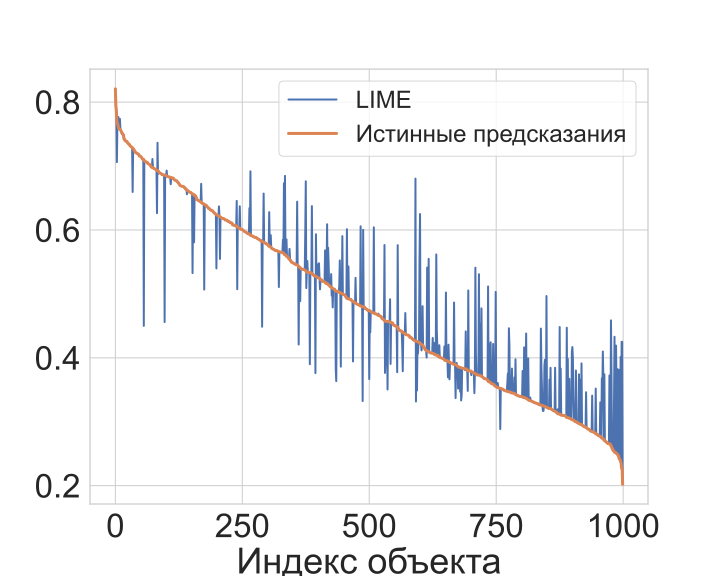
\includegraphics[width=\textwidth]{../figures/lime_proba_est.svg}
% \column{0.5\textwidth}
% 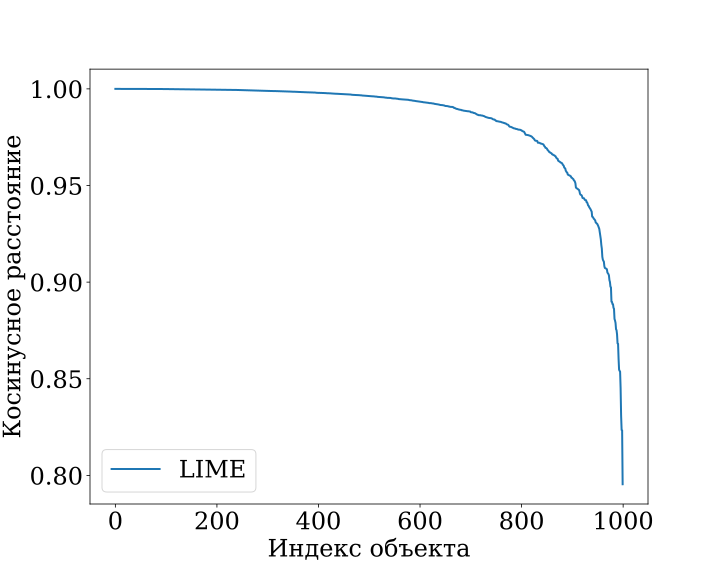
\includegraphics[width=\textwidth]{../figures/lime_cosine.svg}
% \end{columns}
\begin{columns}[c]
\column{0.5\textwidth}
\includesvg[width=\textwidth]{../figures/lime_proba_est.svg}
\column{0.5\textwidth}
\includesvg[width=\textwidth]{../figures/lime_cosine.svg}
\end{columns}
Как видно из графиков, оценки предсказаний, полученные методом LIME значительно отклоняются от истинных для большой доли объектов.

\end{frame}
%----------------------------------------------------------------------------------------------------------
\begin{frame}{Вычислительный эксперимент}
Построим аналогичные графики для метода OpenBox. Напомним, что в данном случае оценивается предсказание модели не в исходном объекте, а в соседнем.
\begin{columns}[c]
\column{0.5\textwidth}
\includesvg[width=\textwidth]{../figures/openbox_proba_est.svg}
\column{0.5\textwidth}
\includesvg[width=\textwidth]{../figures/openbox_cosine.svg}
\end{columns}
\begin{columns}[c]
\column{0.33\textwidth}
\begin{block}{RMSE}
\begin{itemize}
    \item OpenBox: 0.015
    \item LIME: 0.040
\end{itemize}
\end{block}
\column{0.33\textwidth}
\begin{block}{MAE}
\begin{itemize}
    \item OpenBox: 0.008
    \item LIME: 0.014
\end{itemize}
\end{block}
\column{0.33\textwidth}
\begin{block}{MAPE}
\begin{itemize}
    \item OpenBox: 0.019
    \item LIME: 0.039
\end{itemize}
\end{block}
\end{columns}

\end{frame}
%----------------------------------------------------------------------------------------------------------
\begin{frame}{Заключение}
    \begin{itemize}
        \item Предложен метод выбора интерпретируемых рекуррентных моделей с кусочно-линейными функциями активации
        \item Доказана теорема о представлении произвольной рекуррентной нейронной сети в виде математически эквивалентного набора линейных классификаторов
        \item Проведён вычислительный эксперимент, который показал, что предложенный в работе метод обладает более высокой точностью и согласованностью предсказаний, чем ранее известный метод.
    \end{itemize}
\end{frame}
% %----------------------------------------------------------------------------------------------------------
\end{document} 
